%\documentclass{ijsra}
\def\IJSRAidentifier{\currfilebase} %<---- don’t change this!
\def\submission{2017-02-24}%YYYY-MM-DD
\def\acceptance{2017-06-02}%YYYY-MM-DD
%-------Title | Email | Keywords | Abstract-------------
\def\shorttitle{Gendering the traces}
\def\maintitle{Gendering the traces}
\def\cmail{}
\def\keywords{}
%\def\keywordname{}%<--- redefine the name “Keywords“ in needed language
\def\abstract{}
%--------Author’s names------------
\def\authorone{Amanda Padoan}
%-------Biographical information-------------
\def\bioone{}
%------University/Institution--------------
\def\affilone{}

\begin{filecontents}{\IJSRAidentifier.bib}

@Article{bahn1992,
	author       ={Bahn, P.},
	title        ={Bores, Bluffers and Wankas: Some Thoughts on Archaeology and Humor},
	volume       ={11},
	number       ={2},
	pages        ={321},
	date         ={1992},
	journaltitle ={Archaeological Review from Cambridge},
}

@Book{benson2001,
	author       ={Benson, E. and Cook, A.},
	title        ={Ritual Sacrifice in Ancient Peru},
	publisher    ={University of Texas Press},
	date         ={2001},
	location     ={Austin},
}

@Article{emerson2016,
	author       ={Emerson, T.E. and Hedman, K.M. and Hargrave, E.A. and Cobb, D.E.},
	title        ={Paradigms Lost: Reconfiguring Cahokia's Mound 72 Beaded Burial},
	volume       ={81},
	number       ={3},
	pages        ={405--425},
	date         ={2016},
	journaltitle ={American Antiquity},
}

@Book{fowler1977,
	author       ={Fowler, M.},
	title        ={Explorations into Cahokia Archaeology},
	publisher    ={Illinois Archaeological Survey},
    number       ={Bulletin 7},
    edition      ={2},
	date         ={1977},
	location     ={Urbana, IL},
}

@InCollection{fowler1991,
	author       ={Fowler, M.},
	title        ={Mound 72 and Early Mississippian at Cahokia},
	booktitle    ={New Perspectives on Cahokia: Views from the Periphery},
	publisher    ={Prehistory Press},
	editors      ={Stoltman, J. B.},
	date         ={1991},
	series       ={Monographs in World Archaeology}, 
	number       ={2},
	location     ={Madison, WI},
}​

@Book{fowler1999,
	editor       ={Fowler, M. and Rose, J. and {Vander} Leest, B. and Ahler, S.R.},
	title        ={The Mound 72 Area: Dedicated and Sacred Space in Early Cahokia},
	publisher    ={Illinois State Museum Reports of Investigations},
	date         ={1999},
	location     ={Springfield},
}

@Article{hewitt2007,
	author       ={Hewitt, J.},
	title        ={Ethical Components of Researcher-Researched Relationships in Qualitative Interviewing},
	volume       ={17},
	number       ={8},
	pages        ={1153},
	date         ={2007},
	journaltitle ={Qualitative Health Research},
}

@Book{kristeva1982,
	author       ={Kristeva, J.},
	title        ={Powers of Horror: An Essay on Abjection},
	translator   ={Roudiez, L. S.},
	publisher    ={Columbia University Press},
	date         ={1982},
	location     ={New York},
}

@Article{lawson1999,
	author       ={Lawson, T.},
	title        ={Feminism, Realism and Universalism},
	volume       ={5},
	number       ={2},
	pages        ={25--59},
	date         ={1999},
	journaltitle ={Feminist Economics},
}

@URL{macrae2013,
	author   ={Macrae, F.},
	title    ={Drugged with Beer and Cocaine and Left to Freeze to Death, 500-year-old Mummies of Sacrificed Inca Children Reveal their Secrets},
	note={Daily Mail},
	date     ={2013},
	url      ={http://www.dailymail.co.uk/sciencetech/ article-2380813/Incan-children-mummies-Drugged-beer-cocaine-left-freeze-death.html},
	urldate  ={2016-01-30},
}

@URL{osborne2013,
	author   ={Osborne, H.},
	title    ={China: 80 Female Skulls Found in Neolithic City Were Human Sacrifices},
	note={International Business Times},
	date     ={2013},
	url      ={http://www.ibtimes.co.uk/female-skulls-discovered-neolithic-city-china-human-526746},
	urldate  ={2016-01-30},
}

@Book{pauketat1997,
	editor       ={Pauketat, T. and Emerson, T.},
	title        ={Cahokia: Domination and Ideology in the Mississippian World},
	publisher    ={University of Nebraska Press},
	date         ={1997},
	location     ={Lincoln},
}

@Book{rautman2000,
	editor       ={Rautman, A.},
	title        ={Reading the Body: Representations and Remains in the Archeological Record},
	publisher    ={University of Philadelphia Press},
	date         ={2000},
	location     ={Philadelphia},
}

@URL{richards2012,
	author    ={Richards, D.},
	title     ={Girl, 7, is Murdered in India and has Liver Cut Out in Sacrifice to the Gods for a Better Harvest},
	note ={Daily Mail},
	date      ={2012},
	url       ={http://www.dailymail.co.uk/news/article-2081244/Indian-girl-7-murdered-liver-cut-sacrifice-gods-better-harvest.html},
	urldate   ={2016-01-30},
	}

@Article{slater2014,
	author       ={Slater, P. and Hedman, K. and Emerson, T.},
	title        ={Immigrants at the Mississippian Polity of Cahokia: Strontium Isotope Evidence for Population Movement},
	volume       ={44},
	pages        ={117--127},
	date         ={2014},
	journaltitle ={Journal of Archaeological Science},
}

@InCollection{spivak2010,
	author       ={Spivak, G.C.},
	title        ={Can the Subaltern Speak?},
	booktitle    ={Can the Subaltern Speak?: Reflections on the History of an Idea},
	publisher    ={Columbia University Press},
	editors      ={Morris, R.},
	date         ={2010},
	origdate     ={1983},
	location     ={New York},
}

@Article{thompson2013,
	author       ={Thompson, A.},
	title        ={Odontometric Determination of Sex at Mound 72, Cahokia},
	volume       ={151},
	number       ={3},
	pages        ={408--419},
	date         ={2013},
	journaltitle ={American Journal of Physical Anthropology},
}

@Article{thompson2015,
	author       ={Thompson, A. and Hedman, K. and Slater, P.},
	title        ={New Dental and Isotope Evidence of Biological Distance and Place of Origin for Mass Burial Groups at Cahokia’s Mound 72},
	volume       ={158},
	pages        ={341--357},
	date         ={2015},
	journaltitle ={American Journal of Physical Anthropology},
}

@InCollection{weber1946,
	author       ={Weber, M.},
	title        ={Science as Vocation},
	booktitle    ={From Max Weber: Essays in Sociology},
	publisher    ={Oxford University Press},
	editors      ={Gerth, H. H., and Wright Mills, C.},
	date         ={1946},
	location     ={New York},
}
\end{filecontents}
\IJSRAopening%<---- don’t change this!
%-------
\lettrine{A}{bout} thirty years ago, archeologists began examining the archeological record through the lens of modern gender theory. Evolving symbiotically with feminism, the emerging discipline went on to generate innovative analysis. At the same time, gender archeology was playfully derided as \enquote{a new racket for the girls} and ridiculed for \enquote{the empresses' lack of clothes} \parencite[321]{bahn1992}. The silence of the grave had never been more contentious. 

Behind the bombast lurked a valid question: Could we even recognize a prehistoric gender issue if we saw one? At the heart of the problem throbbed fears of theoretical incompatibility. Just as an organ transplanted from one body to another bears the risk of rejection, so too in bodies of knowledge. An interpretative framework conceived in one time may fail or dysfunction in another. Yet situated as we are in time, what's the alternative? Human thought is as perishable as the people producing it and the societies preserving it. Much is lost as the past is filtered through the distortions of a modern mind. A gendered methodology derived from present thought, while never risk-free, is a necessary transplant. 

Loci of human sacrifice are productive sites to examine the tension. One is down an unassuming country road in Illinois. A thousand years ago, the spot witnessed an astonishing amount of bloodshed. Now the Cahokia Mounds make a peaceful picnic spot. Rising above the American Bottom, some offer vistas of downtown St. Louis and just the right incline to tumble down the ramparts as human cannonballs. Frisbees sail over Mound 72, a gentle ripple on the lawn, leveled by successive excavations. Mound 72 is a trace, the memory of a mound, but it towers over the field of gender archeology. Inside, 53 women were found, stacked like matchsticks. All were young, probably teenagers. Isotopes in their tooth enamel don't match those of the Cahokians, so they may have been captives \parencite[]{thompson2013}. Each appears to have been strangled, though not by hand. Manual strangulation fractures a U-shaped bone called hyoid, which anchors the tongue in place, and theirs appear intact. The skeletons present few osteological fractures, no bashed skulls. Someone evidently strangled the girls with a rope or strip of cloth, leaving no trace in bone \parencite[168]{benson2001}. 

Their burial is peripheral to a central grave belonging to an elite man in his 40s. Known as \enquote*{Birdman}, he rests on a falcon-shaped blanket of \num{20000} shell beads \pcref{fig:33-Padoan-figure01}. Five sacrificial retainers crouch beside him and a woman lies beneath him. The 53 matchstick girls share his wider mound but little else. Their remains recall a time, not far removed, when life was cheap and women's lives were cheapest. Birdman died of natural causes; they did not. His life radiates invincibility, proclaiming itself in ways theirs cannot. Beneath Mound 72, Birdman is undiminished. In command of a lost world, he asserts ownership over the semi-precious objects around him: mica, sheet copper, pottery vessels, projectile arrowheads, conch shell beads, and people \parencite[3--8]{fowler1999}. Birdman's clutter is a social declaration, aimed at securing his identity through time.

\begin{figure}[!htb]
	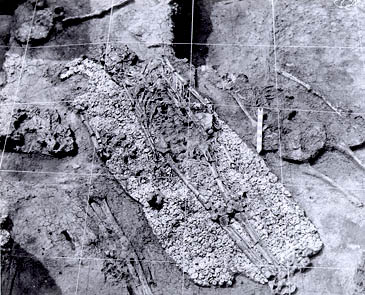
\includegraphics[width=\linewidth]{33-Padoan-figure01}
	\caption{Burial of \enquote*{Birdman}.
		{\normalfont\scriptsize \\ \copyright\ by University of Wisconsin-Milwaukee Archaeological Research Laboratory, used with permission. Cahokia Collection Image 1967.2.31. From \textcite[]{fowler1991}.
	}}
	\label{fig:33-Padoan-figure01}
\end{figure}

In this, he triumphs. His honored life and well-provisioned afterlife practically caw hegemonic exploitation. In Birdman's presence, the pull towards naturalistic fallacy is almost disarticulating. We are told, \begin{IJSRAquote}{\cite[25]{lawson1999}}[t]he practice of universalizing, a priori, of merely asserting/assuming the widespread validity/relevance of some position is now widely recognized as, at best, a methodological mistake\end{IJSRAquote}yet this is a mistake we desperately wish to make. Distilling right from wrong, life from death, power from protest feels reassuring. Still, we are told, when radical feminist values are inferred from trace evidence and left unexamined, methodology breaks down. Our project is to understand as the subjects would have understood without the distraction of moral crisis. As Max Weber cautions, the descent into value-laden science comes at a cost: \begin{IJSRAquote}{\cite[146]{weber1946}}Whenever the person of science introduces his personal value judgment, a full understanding of the facts ceases.\end{IJSRAquote}Gender archeology might thus be reduced to live women saving dead women from dead men.\footnote{Recalling Spivak's evocative phrase about the dysfunctions of salvationist feminism: \begin{IJSRAquote}{\cite[48]{spivak2010}}White men are saving brown women from brown men.\end{IJSRAquote}} Besides, it's too late for them. Inside Mound 72, lived experience is dead and gone. Who can be saved now? If not them, then us.

Sites like Mound 72 are politically charged forums in part because they echo present-day concerns about gender violence. Indeed, there is widespread interest in ancient atrocity, suggesting gender violence is safer to confront when it is long passed and demands nothing by way of intervention. In such cases, we are free to empathize without the burden of action or the guilt of inaction. These archeological discoveries have a license to thrill, titillate and make headlines: \begin{IJSRAquote}{\cite[]{osborne2013}}[S]kulls of 80 women who were used as human sacrifices... used to build the city walls\end{IJSRAquote}blasts the International Business Times. Four thousand years on, their deaths are our business. \enquote{Drugged with Beer and Cocaine and Left to Freeze to Death} runs a Daily Mail exposé of a 13 to 15-year-old Incan girl whom archeologists christened \enquote{La Doncella} \parencite[]{macrae2013}. Sacrificed some 500 years ago on an icy volcano, she is now the star of National Geographic's Child Mummy Sacrifice DVD Exclusive, which is often sold out. This forensic drama spans the last year of her life as hair proteins reveal a switch from maize to meat and she is plumped for the kill. 

La Doncella's ordeal is infamous. Another is more obscure. In 2012, Lalita Tati, a 7-year-old girl from Jailwara, India, was abducted by two farmers. The men slit her throat, removed her heart and liver, and offered them to the Hindu goddess Durga \parencite[]{richards2012}. Rainfall had been scarce, and Lalita's organs, the killers later confessed, were needed to bless the harvest. Strategically, the men reframed their butchery as a sacrifice for the benefit of the community. Murder, thus reimagined, became an act of regeneration. But their sacrificial intent was suspect. Neither man's livelihood depended on the land's productivity. In fact, before the murder they were feuding with Lalita's father. What is extraordinary about this killing is neither its cruelty nor its perversity, but how human sacrifice is still used reflexively to conceal motive. It is a defense strategy with ancient roots and contemporary relevance. In power grabs large and small, the female body is exposed, marked and, in Lalita's case, gutted. So long as girls like Lalita Tati are being murdered as a form of masculine assertion, Mound 72 can never be ancient history. 

Gender violence is uniquely demonstrative. Even as the concept of gender resists essentializing over time, violence offers no such resistance. Even as our diverse choreographies of violence evolve, killing proceeds as it always has. Could the intersection between the constancy of violence and fluidity of gender elucidate both categories? In Mound 72, power relations are marked in fractured vertebrae. Social control is deduced from the absence of breaks in the radii and ulnae, bones of the lower arm that deflect blows. An absence of defensive injuries indicates bodies well under control at time of death. These girls didn't fight back. The temptation is to do it for them. Indeed, a gendered methodology must fight back in certain ways. Archaeology cut its teeth in cultural theft and once produced arbitrary analysis, reflecting the motley agendas of its investigators. When Heinrich Schliemann unearthed golden diadems at Hissarlik, the putative site of Troy, he considered the find dazzling enough to grace 'the face that launched a thousand ships.' No matter the surrounding sediment was deposited a millennium before the Trojan War. Schliemann wanted the diadems to be the Jewels of Helen. So they were, even if they weren't. When he draped the glittering chains and tassels over his 21-year-old wife, Sophia, a version of Helen revived. His error was spectacularly photogenic. To illustrate the fallacy of wishful thinking, one need only turn to the epic snapshot. Sophia Schliemann’s face, captured in tintype, launches a thousand questions. Beneath the gold fringe, her gaze is fixed as though she too sees her husband's claims are absurd, a gendered methodology gone wrong. 
%Schliemann source quote needed here

How, then, to avoid Schliemann's mistake of misrepresenting the gendered subject? Gender, rife with codes and inconsistencies, is elusive enough in the present, let alone the past. At least Schliemann had Homer to confuse him. Prehistory leaves no surviving texts and only whispers of an oral tradition. Instead, the contours of gender must be traced in the visual and material culture. How a body is adorned, positioned, bound and broken animates the gendered subject. In practice, however, a gendered methodology often makes assumptions about the female body that undermine Weber's mission for a 'full understanding of the facts.' By way of illustration, 'gender violence' is the term most archeologists use in place of 'violence against women' because many skeletons cannot be sexed with certainty. In the skeletal analysis of Mound 72, for example, \begin{IJSRAquote}{\cite[63]{fowler1999}}sex classes are: \num{-2} hyperfeminine, \num{-1} feminine, \num{0} indifferent, +1 masculine, +2 hypermasculine.\end{IJSRAquote} To populate the negative range, archeologists seek \enquote{the gracile features characteristic of females} \parencite[54]{fowler1999}. Although sex is uncertain, the perceived gender for these fifty-three skeletons becomes inexorably feminine or hyperfeminine. 

%quote source needed for Weber's 'full understanding of the facts'

An all-female hypothesis for the 53 skeletons prevailed for decades and not for strictly scientific reasons. This perception is changing. In 2015, a new study reanalyzed the skeletal material from Mound 72 and challenged long-held assumptions about these women \parencite[]{slater2014}. For one thing, some may not be women at all. Based on dental metrics, a few deceptively gracile men slipped into the mix \parencite[]{thompson2013}. A methodology sensitive to the nuances of gender might have detected this sooner. To avoid the normative pitfalls of sex and gender differentiation, \begin{IJSRAquote}{\cite[3]{rautman2000}}it is more productive to consider sexual/gender categories as gradational.\end{IJSRAquote} A presumption of gender ambiguity and fluidity is the better methodology in a mortuary context. 

Organization, too, can be deceptive. Inside Mound 72, the placement is meticulous, recalling Julia Kristeva's observation that, \begin{IJSRAquote}{\cite[102]{kristeva1982}}the body must bear no trace of its debt to nature: it must be clean and proper to be fully symbolic.\end{IJSRAquote} Perhaps this is why Lalita Tati failed to capture the popular imagination. Organs displaced, Lalita embodies disorganization. She is messy in a way bare bones can never be. In contrast, time and decomposition transfigure the girls of Mound 72, elevating their remains to a concept. Whatever their experience with violent death, now they're too clean for comparison. No trace remains of the struggle to survive. They rest in quiet symmetry, shelves of compliant girls, banded by woven reeds. An explanation should be as neat as they are. But it isn't, because they are human, and so are we. We know their hearts once beat, their minds circled, their breath ceased as the garrote winched. Even as we are told, \begin{IJSRAquote}{\cite[1153]{hewitt2007}}Research outcomes, at best, represent only a version of the truth [and] cannot be said to describe the lived experience of another\end{IJSRAquote} we struggle alongside them. We struggle with a method that denies us the visceral response. 

\IJSRAclosing%<---- don’t change this!